\documentclass{beamer}

\usepackage{amsthm}
\usepackage[utf8]{inputenc}
\usepackage[T1]{fontenc}
\usepackage[brazil]{babel}
\usepackage[export]{adjustbox}
\usepackage{listings}
\usepackage{fontspec}
\usepackage{color}

\definecolor{pblue}{rgb}{0.13,0.13,1}
\definecolor{pgreen}{rgb}{0,0.5,0}
\definecolor{pred}{rgb}{0.9,0,0}
\definecolor{pgrey}{rgb}{0.46,0.45,0.48}

\lstset{language=Java,
  showspaces=false,
  showtabs=false,
  breaklines=true,
  showstringspaces=false,
  breakatwhitespace=true,
  commentstyle=\color{pgreen},
  keywordstyle=\color{pblue},
  stringstyle=\color{pred},
  basicstyle=\ttfamily,
}


\usetheme{Madrid}
\usecolortheme{beetle}
\usefonttheme{professionalfonts}

\setmainfont{Oswald}

\lstset{basicstyle=\ttfamily,breaklines=true}
\beamertemplatenavigationsymbolsempty

\begin{document}

\selectlanguage{brazil}
\title[Pilhas e Filas]{Pilhas e Filas}
\author{Prof. Andrey Masiero}

\begin{frame}[plain,noframenumbering]
  \titlepage
\end{frame}

\begin{frame}[plain,noframenumbering]
  \frametitle{Agenda}
  \tableofcontents
\end{frame}

\section{Introdução}

\begin{frame}
	\frametitle{Introdução}
    \begin{itemize}
        \item São conjuntos dinâmicos para armazenar informações;
        \item A informação removida é especificada previamente a sua implementação.
    \end{itemize}
\end{frame}

\begin{frame}
	\frametitle{Introdução}
    \begin{block}{Pilha}
        \begin{itemize}
            \item o elemento removido é o mais recente;
            \item Esse tipo de operação é conhecida como \textbf{LIFO} (\textit{Last In, First Out}).
        \end{itemize}
	\end{block}

    \begin{block}{Fila}
        \begin{itemize}
            \item o elemento removido é o mais antigo;
            \item Esse tipo de operação é conhecida como \textbf{FIFO} (\textit{First In, First Out}).
        \end{itemize}
	\end{block}
\end{frame}

\section{Pilha}

\begin{frame}
	\begin{center}
        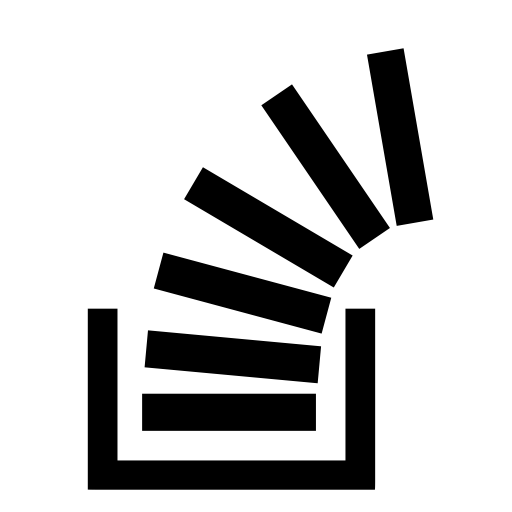
\includegraphics[scale=0.2]{images/stack.png}

		\Huge Pilha
	\end{center}
\end{frame}

\begin{frame}
	\frametitle{Pilha}
    \begin{table}
        \caption{Operações básicas de Pilha}
        \label{tab:pilha}
        \begin{tabular}{| c | c |}
            \hline
            Operação & Descrição \\ \hline
            \texttt{push} & Insere um novo valor na pilha \\ \hline
            \texttt{pop} & Remove um valor da pilha \\ \hline
            \texttt{top} & Consulta o valor no topo da pilha \\ \hline
            \texttt{isEmpty} & Verifica se a pilha está vazia \\ \hline
        \end{tabular}
    \end{table}
\end{frame}

\begin{frame}
	\frametitle{push}
    \centering
    \lstinputlisting[language=Java]{src/push.java}
\end{frame}

\begin{frame}
	\frametitle{pop}
    \centering
    \lstinputlisting[language=Java]{src/pop.java}
\end{frame}

\begin{frame}
	\frametitle{top}
    \centering
    \lstinputlisting[language=Java]{src/top.java}
\end{frame}

\begin{frame}
	\frametitle{isEmpty}
    \centering
    \lstinputlisting[language=Java]{src/vazio_pilha.java}
\end{frame}

\section{Fila}

\begin{frame}
	\begin{center}
        
\includegraphics[scale=0.1]{images/queue.png}

		\Huge Fila
	\end{center}
\end{frame}

\begin{frame}
	\frametitle{Fila}
    \begin{table}
        \caption{Operações básicas de Fila}
        \label{tab:fila}
        \begin{tabular}{| c | c |}
            \hline
            Operação & Descrição \\ \hline
            \texttt{enqueue} & Insere um novo valor na fila \\ \hline
            \texttt{dequeue} & Remove um valor da fila \\ \hline
            \texttt{front} & Consulta o valor no início da fila \\ \hline
            \texttt{isEmpty} & Verifica se a fila está vazia \\ \hline
        \end{tabular}
    \end{table}
\end{frame}

\begin{frame}
	\frametitle{enqueue}
    \centering
    \lstinputlisting[language=Java]{src/enqueue.java}
\end{frame}

\begin{frame}
	\frametitle{dequeue}
    \centering
    \lstinputlisting[language=Java]{src/dequeue.java}
\end{frame}

\begin{frame}
	\frametitle{front}
    \centering
    \lstinputlisting[language=Java]{src/front.java}
\end{frame}

\begin{frame}
	\frametitle{isEmpty}
    \centering
    \lstinputlisting[language=Java]{src/vazio_fila.java}
\end{frame}

\section{Exercícios}

\begin{frame}
    \frametitle{Exercícios}
    \begin{enumerate}
        \item Implemente uma Pilha utilizando vetor (sequencial/estática).
        \item Implemente uma Fila utilizando vetor (sequencial/estática).
        \item Implemente uma Pilha utilizando vetor (encadeada/dinâmica).
        \item Implemente uma Fila utilizando vetor (encadeada/dinâmica).
        \item Faça um programa que teste todas as estruturas criadas.
    \end{enumerate}
\end{frame}

\section{Referências}

\begin{frame}
    \frametitle{Referências Bibliográficas}
    \begin{enumerate}
        \item Cormen, Thomas H., Charles E. Leiserson, Ronald L. Rivest, and Clifford Stein. ``Introduction to algorithms second edition.'' (2001).
        \item Tamassia, Roberto, and Michael T. Goodrich. ``Estrutura de Dados e Algoritmos em Java.'' Porto Alegre, Ed. Bookman 4 (2007).
        \item Ascencio, Ana Fernanda Gomes, and Graziela Santos de Araújo. ``Estruturas de Dados: algoritmos, análise da complexidade e implementações em JAVA e C/C++.'' São Paulo: Perarson Prentice Halt 3 (2010).
    \end{enumerate}
\end{frame}

\end{document}
